%%%%%%%%%%%%%%%%%%%%%%%%%%%%%%%%%%%%%%%%%%%%%%%%%%%%%%%%%%%%%%%%%%%%%%%%%%%%%%%%
\documentclass[presentation]{beamer} %\mode<presentation>{\usetheme{sapere}}
\usetheme{CambridgeUS}
\usecolortheme{orchid}

\definecolor{themeColor}{HTML}{11AD1E}

\setbeamercolor*{structure}{bg=black,fg=themeColor}

\setbeamercolor*{palette primary}{use=structure,fg=white,bg=structure.fg}
\setbeamercolor*{palette secondary}{use=structure,fg=white,bg=structure.fg!75}
\setbeamercolor*{palette tertiary}{use=structure,fg=white,bg=structure.fg!50!black}
\setbeamercolor*{palette quaternary}{fg=white,bg=black}

\setbeamercolor{section in toc}{fg=black,bg=white}
\setbeamercolor{alerted text}{use=structure,fg=structure.fg!50!black!80!black}

\setbeamercolor{titlelike}{parent=palette primary,fg=structure.fg!50!black}
\setbeamercolor{frametitle}{bg=structure.fg!10!white,fg=structure.fg!50!black!80!black}

\setbeamercolor*{titlelike}{parent=palette primary}

\usepackage[utf8]{inputenc}
\usepackage{amssymb}
\usepackage{graphicx}
\usepackage{subfigure}
\usepackage{multirow}
\usepackage{hhline}
\usepackage{amsfonts,amstext,amssymb,wasysym}
\usepackage{fancyvrb}
\usepackage{alltt}
\usepackage{textcomp}
\usepackage{url}
\usepackage{multimedia,pgf}
\usepackage{geometry}
\usepackage{listings}
\usepackage{bibentry}
\usepackage{framed}
\usepackage{cleveref}
\nobibliography*

% Code highlighting
\definecolor{Fuchsia}{HTML}{8C368C}
\definecolor{OliveGreen}{HTML}{3C8031}

\newcommand{\il}[1]{{\it \textcolor{gray}{// #1}}} % inline comment
\newcommand{\km}[1]{\textcolor{purple}{#1}} % key mechanism primitives
\newcommand{\ex}[1]{\textcolor{blue}{#1}} % external imported Java values
\newcommand{\fc}[1]{\textcolor{Fuchsia}{#1}} % field calculus calls
\newcommand{\fn}[1]{\textcolor{blue}{#1}} % building block / function calls
\newcommand{\vb}[1]{\textcolor{OliveGreen}{#1}} % variables
\newcommand{\str}[1]{\textcolor{darkgray}{#1}} % strings

\newcommand{\bral}{\textrm{{\tt {\char '173}}}\,}
\newcommand{\brar}{\textrm{{\tt {\char '175}}}}
\newcommand{\var}{\texttt{x}}
\newcommand{\asgK}{~\texttt{=}~}
\newcommand{\letK}{\texttt{let}~}
\newcommand{\tupK}[1]{\texttt{[}#1\texttt{]}}
\newcommand{\lambdaK}[2]{\texttt{(}#1\texttt{)->}#2}
\newcommand{\bodyK}[1]{\bral\! #1\!\brar}
\newcommand{\dotK}{\texttt{.}}
\newcommand{\applyK}{\texttt{apply}}
\newcommand{\mname}{\ex{\texttt{m}}}
\newcommand{\aname}{\ex{\texttt{\#a}}}
\newcommand{\repK}[3]{\texttt{\fc{rep}(#1<-#2)}#3}
\newcommand{\ifK}[3]{\texttt{\fc{if}}(#1)#2\,\texttt{\fc{else}}\,#3}
\newcommand{\muxK}[3]{\texttt{\fc{mux}}(#1)#2\,\texttt{\fc{else}}\,#3}
\newcommand{\nbrK}[1]{\texttt{\fc{nbr}}#1}


\title[Computational Fields and Augmented Reality]{Computational Fields meet Augmented Reality: Perspectives and Challenges}

\author[Pianini et. al]{
Danilo Pianini, Angelo Croatti, Mirko Viroli, Alessandro Ricci\\
\texttt{{\footnotesize \{danilo.pianini, a.croatti, mirko.viroli, a.ricci\}@unibo.it}}}


\institute[UniBo]
{\textsc{Alma Mater Studiorum}---Universit\`a di Bologna a Cesena}

\date[2015-09-21 SCOPES]{Spatial and COllective PErvasive Computing Systems (SCOPES)\\
\scriptsize September 21, 2015 - Cambridge, USA
}

\pgfdeclareimage[height=0.625cm]{university-logo}{images/logo}
\logo{\pgfuseimage{university-logo}}


\begin{document}

\AtBeginSubsection[]{%
  \begin{frame}<beamer>
    \frametitle{Outline}
    \tableofcontents[currentsection,currentsubsection]
  \end{frame}
  \addtocounter{framenumber}{-1}% If you don't want them to affect the slide number
}

%===============================================================================
\frame[label=coverpage]{\titlepage}
%===============================================================================

\section*{Outline}
%===============================================================================
\frame{\tableofcontents}

%===============================================================================
\section{Introduction}
%===============================================================================

\subsection{Motivation}
\begin{frame}{Why Augmented Reality and Computational Fields?}
  \begin{block}{Differences}
    They are definitely different entities
    \begin{itemize}
      \item CF is a programming abstraction. AR is a mean of interaction.
      \item CF focuses on collectivity, AR (mostly) on the single user.
    \end{itemize}
  \end{block}
  \begin{block}{Commonalities}
    They share a common context of application
    \begin{itemize}
      \item Both are devoted at environments pervaded with computational devices
      \item Both are bound to the physical world
    \end{itemize}
  \end{block}
\end{frame}


%===============================================================================
\section{Augmented Reality}
%===============================================================================
%-------------------------------------------------------------------------------
\subsection{Basics}
%-------------------------------------------------------------------------------
\begin{frame}{Definition}
  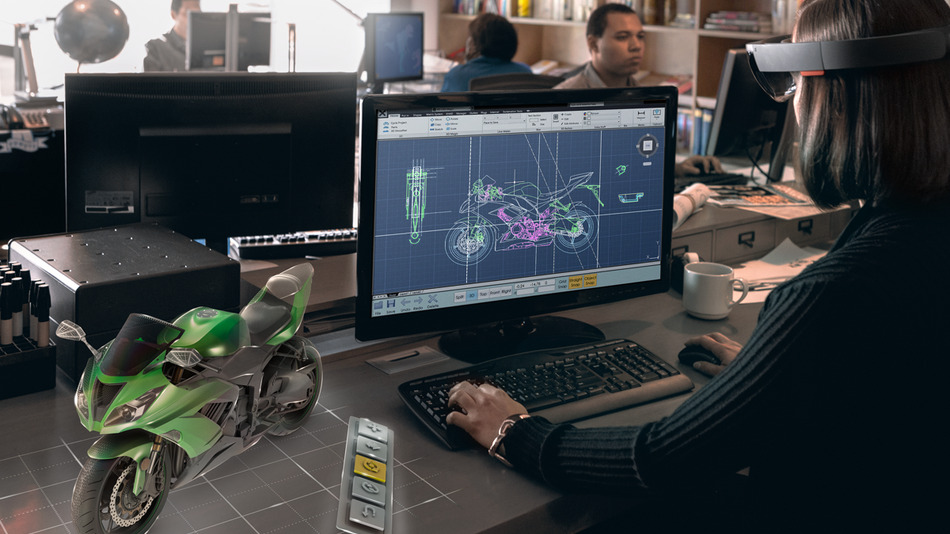
\includegraphics[width=.49\textwidth]{images/holobike}
  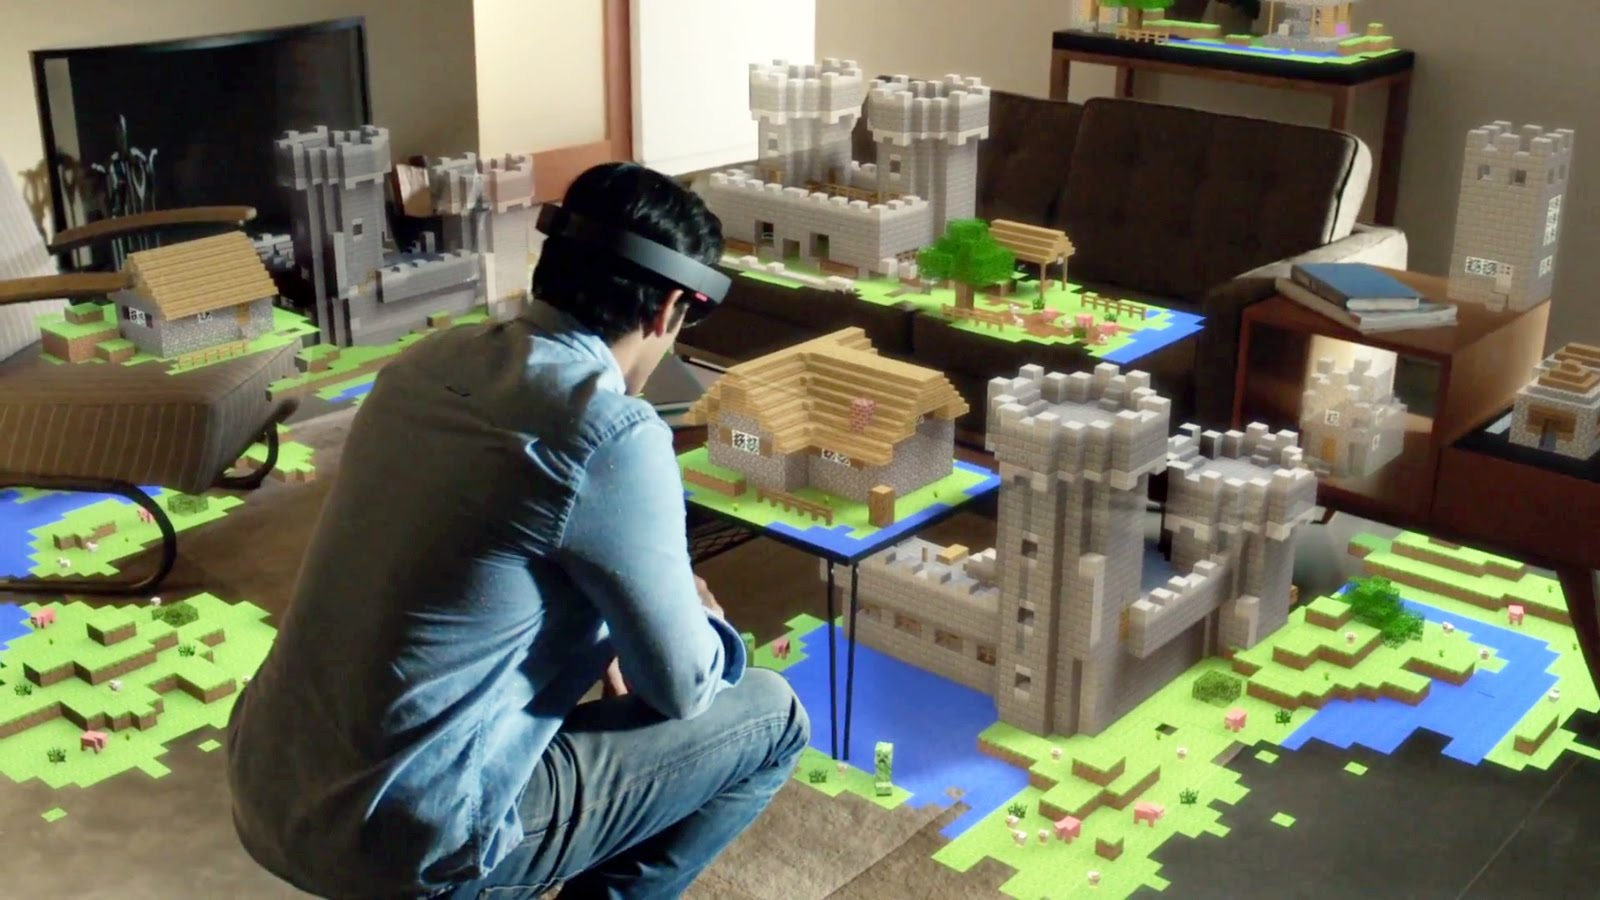
\includegraphics[width=.49\textwidth]{images/holominecraft}
  \begin{block}{Augmented Reality}
    is a technology that allows the user to see the \textbf{real world, with virtual objects} superimposed upon or mixed with the real world \cite{Azuma97}.
    \begin{itemize}
      \item The ultimate goal is a seamless integration of reality and virtuality
      \item Mostly via see-through devices
    \end{itemize}
  \end{block}
  \begin{center}
    \tiny{Images from Microsoft Hololens presentation video}
  \end{center}
\end{frame}

\begin{frame}{Degrees of augmentation}
  \begin{center}
    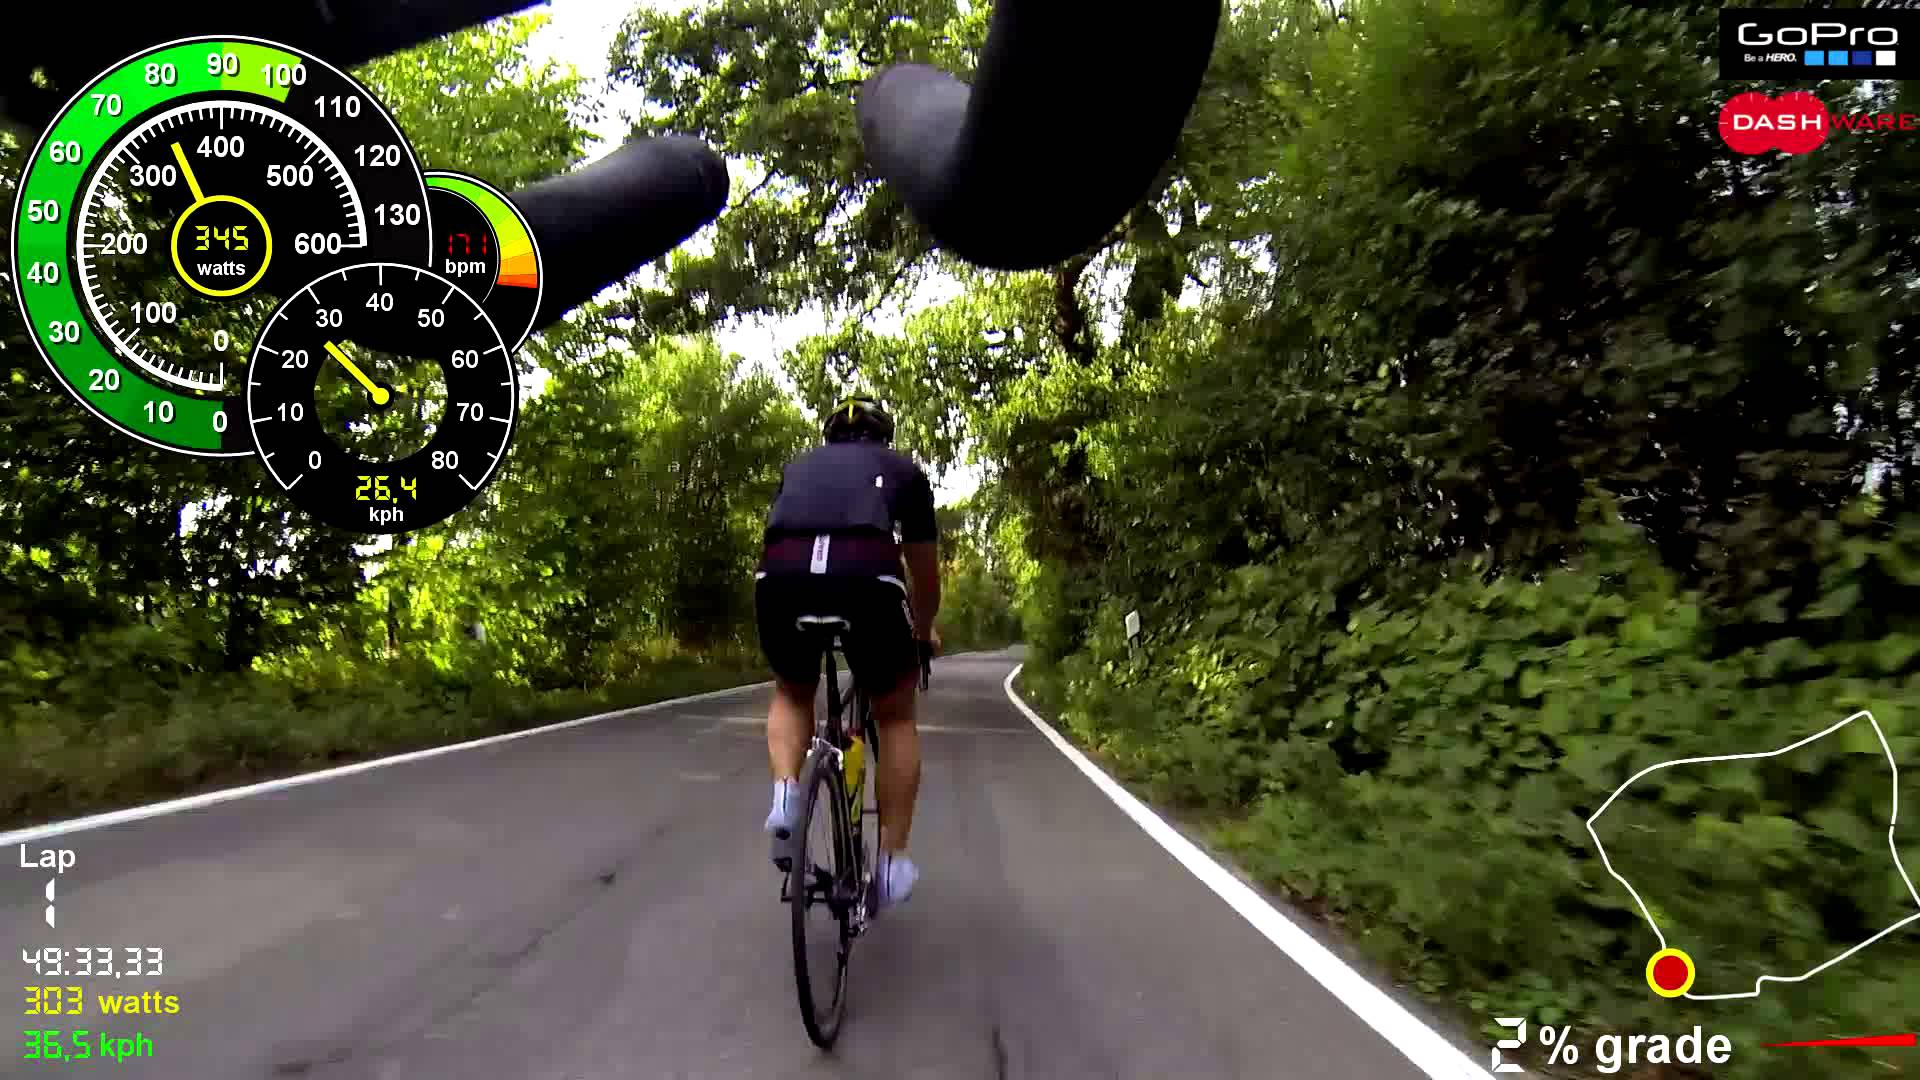
\includegraphics[height=.2\textwidth]{images/dashware}
    ~
    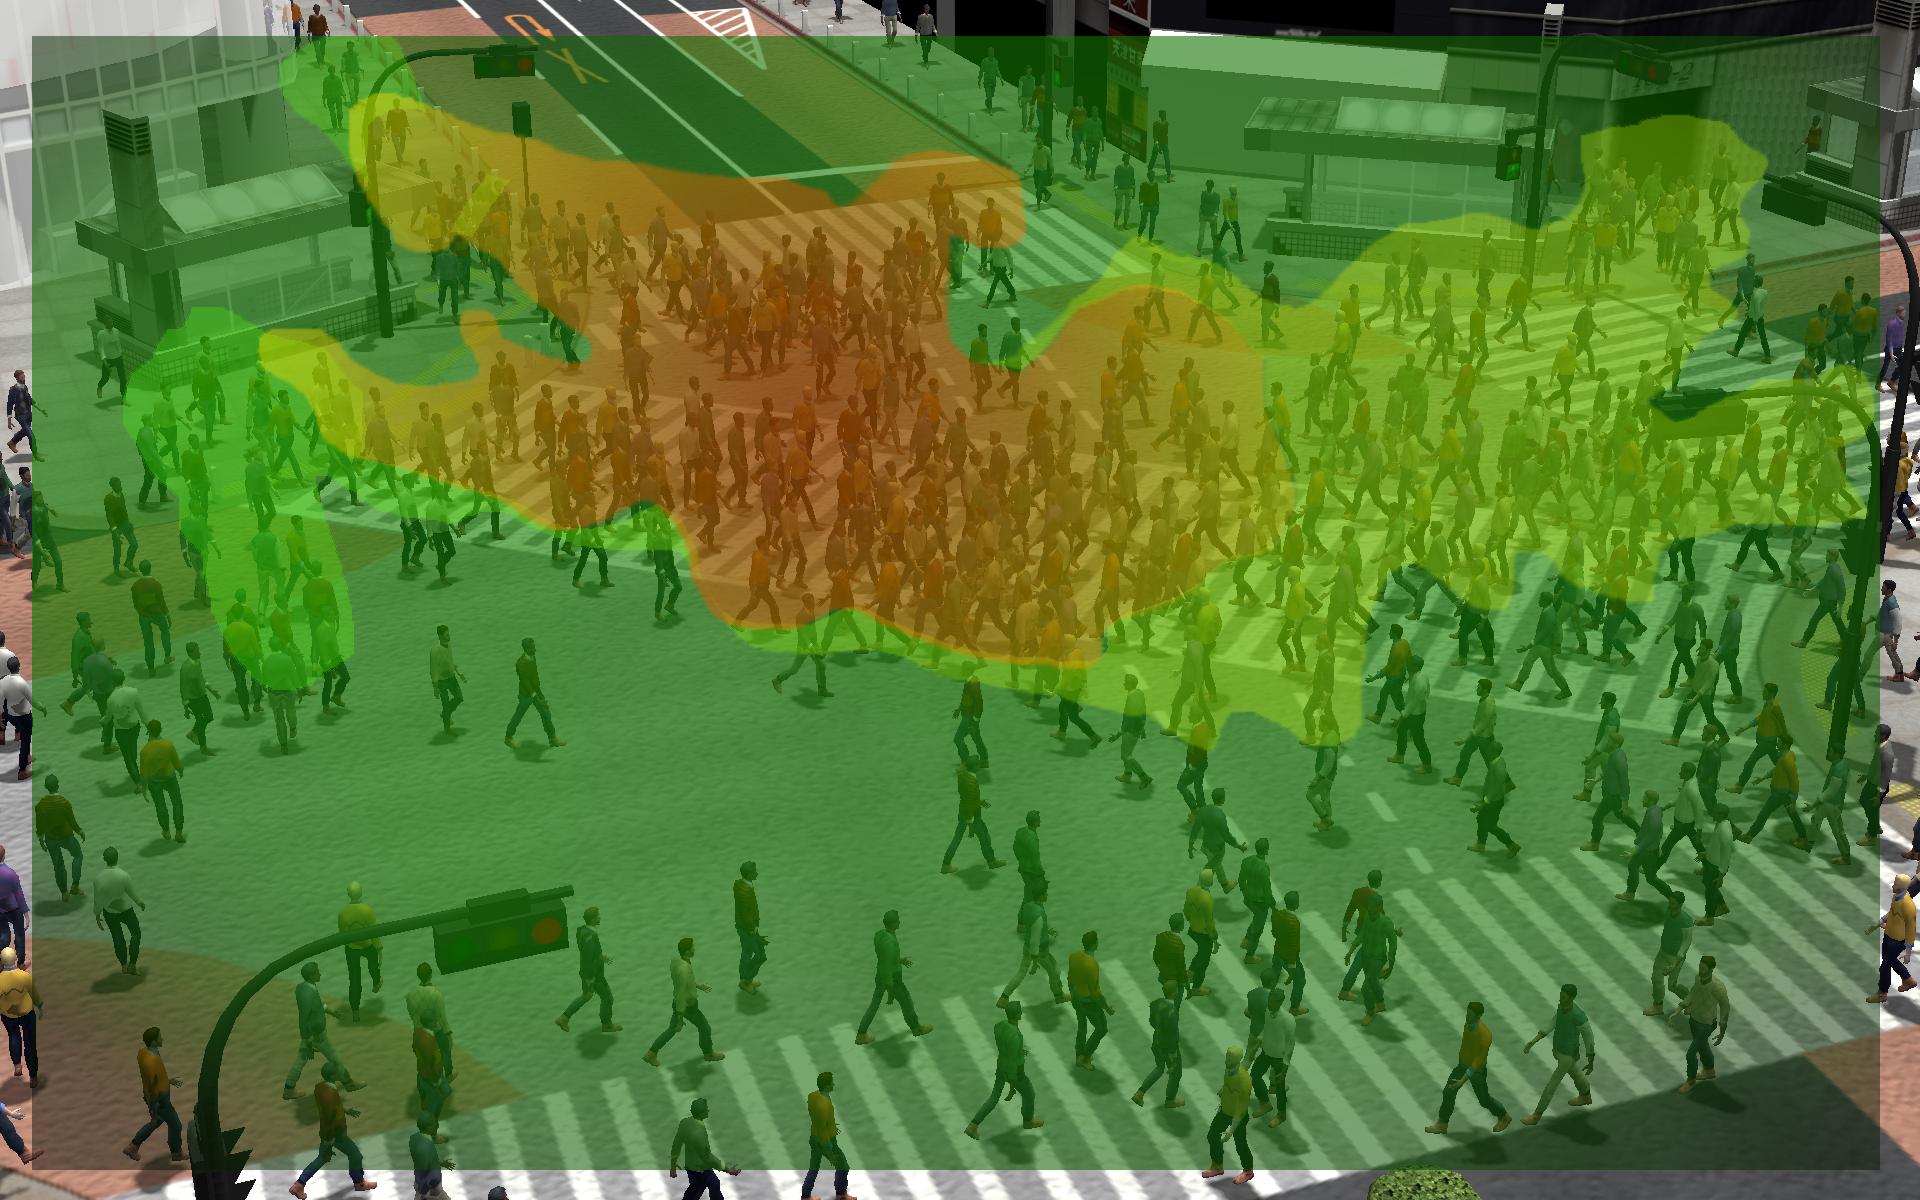
\includegraphics[height=.2\textwidth]{images/crowd01}
    ~
    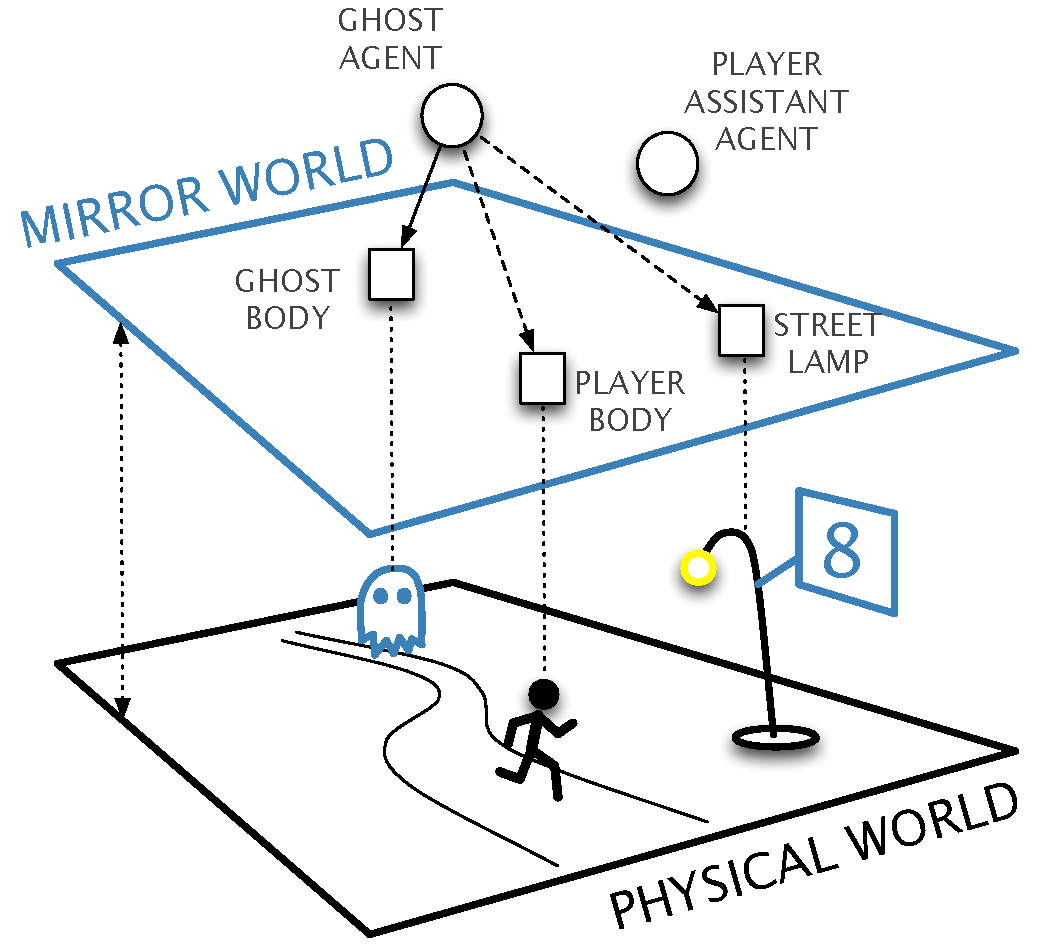
\includegraphics[height=.2\textwidth]{images/game2}
  \end{center}
  Augmentation can happen at different levels:
  \begin{enumerate}
    \item \textbf{Unrelated} to the elements in the user's FOV
      \begin{itemize}
        \item E.g. displaying a map on a visual overlay
      \end{itemize}
    \item \textbf{Dynamically associated} to elements in the user's FOV
      \begin{itemize}
        \item E.g. displaying historical information next to a monument in FOV
      \end{itemize}
    \item \textbf{Entirely virtual and interactive} elements on real world
      \begin{itemize}
        \item E.g. the two images of the previous slide, the ghost game \cite{MirrorWorlds}
      \end{itemize}
  \end{enumerate}
  \begin{center}
    \tiny{Images from (left to right): DashWare, BOH, \cite{MirrorWorlds}}
  \end{center}
\end{frame}

%===============================================================================
\section{Computational fields}
%===============================================================================
%-------------------------------------------------------------------------------
\subsection{Introduction to aggregate programming and computational fields}
%-------------------------------------------------------------------------------
\begin{frame}{Manifesto of aggregate computing}
  \begin{block}{Main observation}
    In a world with ever increasing number of deployed devices, one conveniently views a dense aggregation of interacting devices as a discrete approximation of the space of computational environment through which they are distributed.
  \end{block}
  \begin{center}
    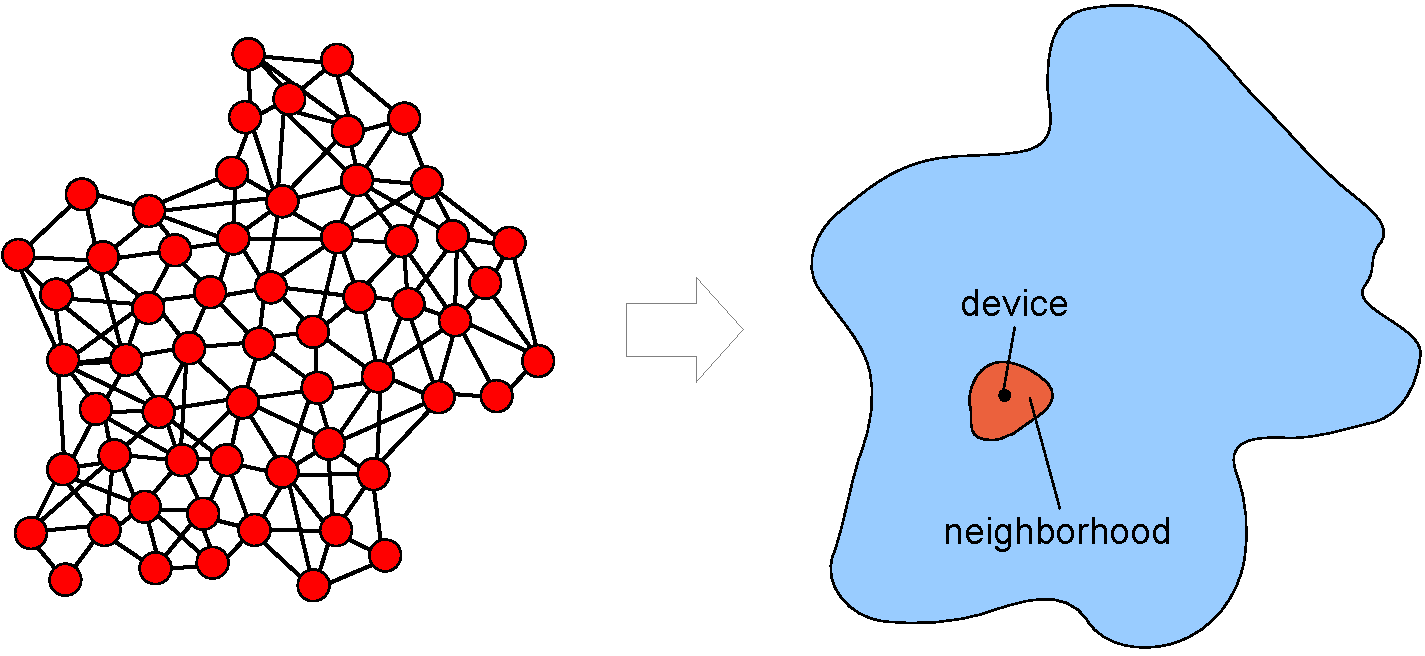
\includegraphics[width=.65\textwidth]{images/amorphous.pdf}
  \end{center}
\end{frame}

\begin{frame}{Manifesto of aggregate computing}
  \begin{block}{Main observation}
    \begin{enumerate}
      \item the reference ``machine'' for pervasive computing processes is abstracted to be the continuum of computational devices;
      \item the reference ``elaboration process'' is the manipulation of a physically distributed data structure;
      \item how computation is carried on by the cooperation of devices in that region is hidden ``under-the-hood'' of the model/platform
    \end{enumerate}
  \end{block}
  \begin{center}
    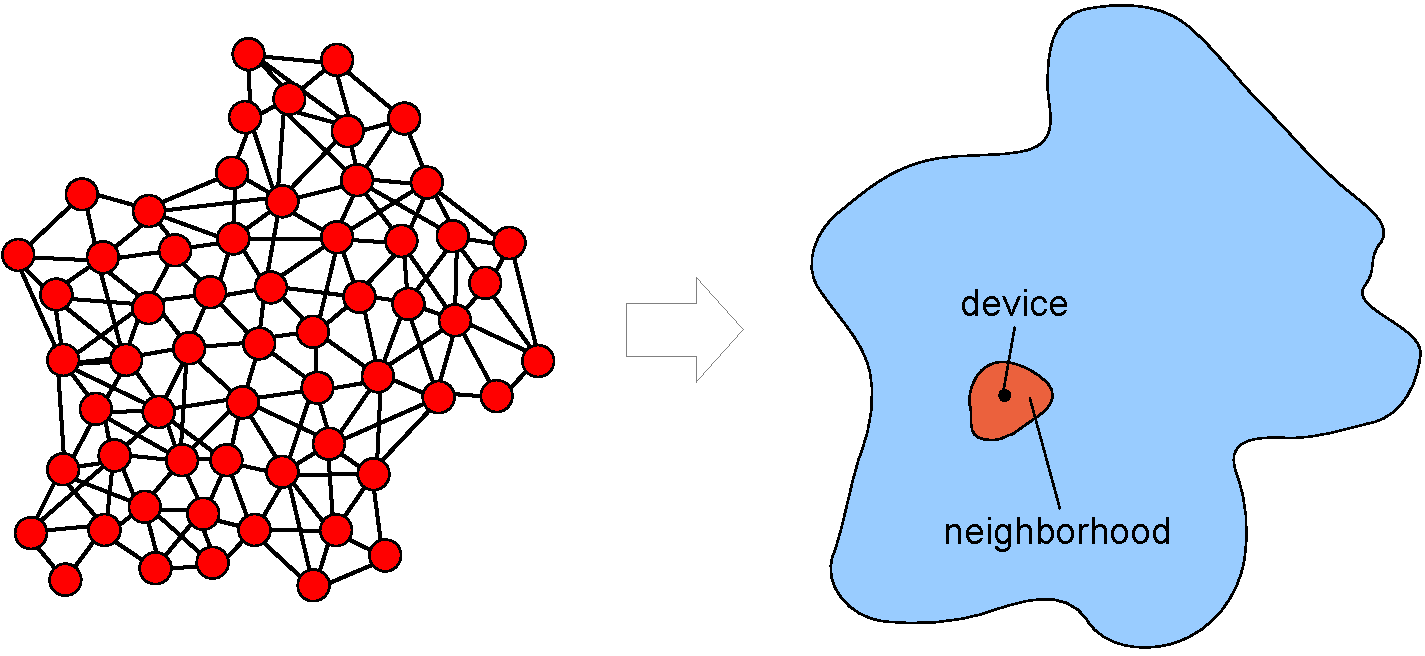
\includegraphics[width=.65\textwidth]{images/amorphous.pdf}
  \end{center}
\end{frame}

\begin{frame}{Pervasive continuum and computational fields}
  \begin{block}{Aggregate computing}
    \begin{itemize}
      \item From ``what value the single device computes''...
      \item ...to ``what distributed data structure the pervasive fabric computes''
      \item The notion of \alert{computational field} arises \cite{tota,beal}
      \begin{itemize}
        \item[$\Rightarrow$] a map from the space to (structured) values
        \item typically evolving over time, possibly self-stabilising
        \item better ``understood'' on continuous domains
      \end{itemize}
    \end{itemize}
  \end{block}
  \begin{center}
    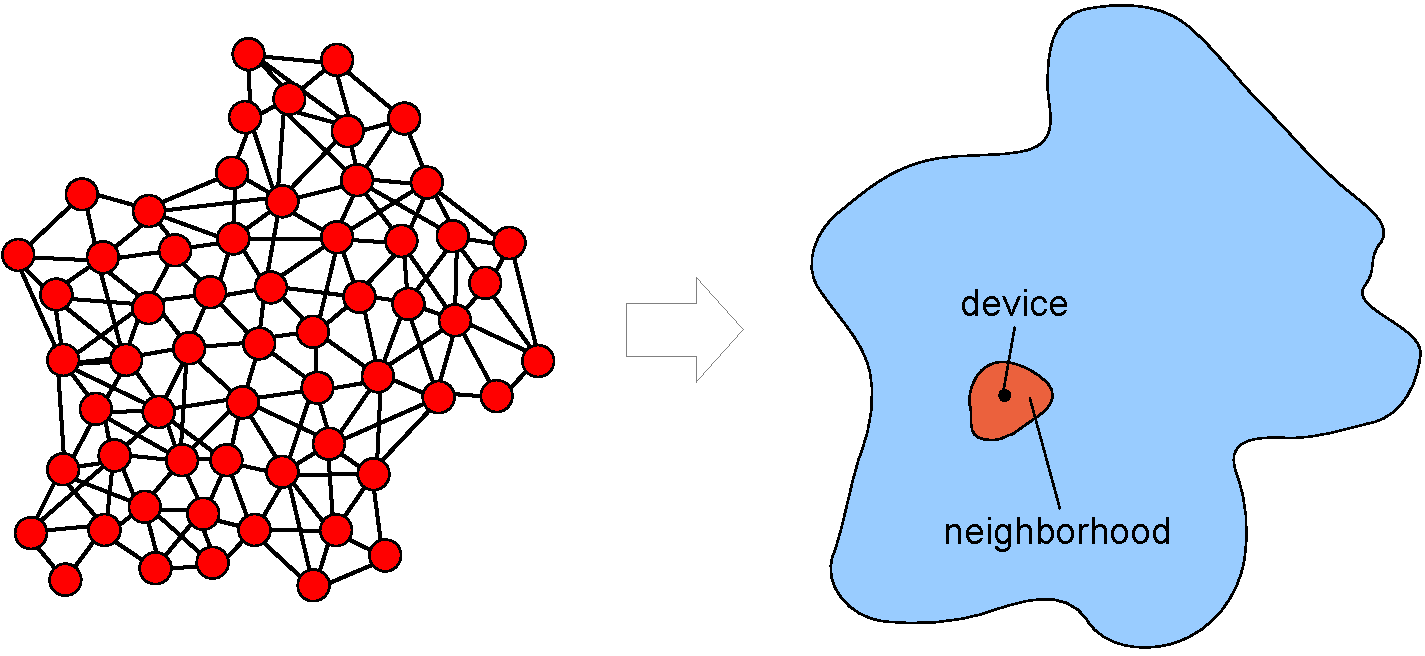
\includegraphics[width=.65\textwidth]{images/amorphous.pdf}
  \end{center}
\end{frame}

%-------------------------------------------------------------------------------
\subsection{Languages for aggregate computing}
%-------------------------------------------------------------------------------

\begin{frame}[fragile]{Existing languages}
  \begin{block} {MIT Proto \cite{beal} is the most known and successful}
   \begin{itemize}
    \item Developed at MIT and maintained at BBN Technologies
    \item Functional language, LISP-like syntax (I know you hate it too)
    \item \emph{All devices run the same program}
    \item Computation happens in rounds:
    \begin{itemize}
      \item Every device sleeps for some time
      \item Processes the messages received from the neighbours
      \item Executes its program
      \item Sends all the neighbours its result
    \end{itemize}
    \item Complex operational semantics
    \item Difficult to maintain and extend 
   \end{itemize}
  \end{block}
\end{frame}

\begin{frame}[fragile]{Field Calculus}
  \begin{block} {A ``distillate'' of Proto}
   \begin{itemize}
    \item Provides a lightweight operational semantics \cite{VDB-FOCLASA-CIC2013}
    \item ((((LISP-like syntax))))
    \item Still a functional language
    \item Simple enough to formally prove properties, powerful enough to be universal (proved!)
    \item Theoretical object, no runtime nor simulation tool provided
   \end{itemize}
  \end{block}
\end{frame}

\begin{frame}{Protelis \cite{ProtelisSAC14}}
  \begin{block} {Ordinary language features}
   \begin{itemize}
    \item Functional language
    \item Same operational semantics of the field calculus 
    \item C-family syntax with infix operators
    \item \underline{Java interoperability}: static methods imports and calls, method invocation with dynamic binding
    \item \underline{Higher order functions} (functions as arguments, lambdas)
    \item Dynamic code
   \end{itemize}
  \end{block}
  \begin{block} {Suggested read \cite{IoT2015}}
     \bibentry{IoT2015}
  \end{block}
\end{frame}

\begin{frame}[fragile]{Code example}
\begin{Verbatim}[fontsize=\scriptsize, frame=single, commandchars=\\\{\}]
\km{def} \fn{count}() \{
   \repK{\vb{\var}}{0} {\bodyK{\vb{\var} + 1\; } }
\}

\km{def} \fn{maxh}(\vb{field}) \{ \fc{maxHood}(\nbrK{(\vb{field})}) \}

\km{def} \fn{distanceTo}(\vb{source}) \{
   \fc{rep} (\vb{d} <- \fc{Infinity}) \{
      \fc{mux} (\vb{source}) \{ 0 \} \fc{else} \{ \fc{minHood}(\fc{nbr}(\vb{d}) + \fc{nbrRange}) \}
   \}
\}

\km{def} \fn{distanceToWithObstacle}(\vb{source}, \vb{obstacle}) \{
   \fc{if} (\vb{obstacle}) \{ \fc{Infinity} \} \fc{else} \{ \fn{distanceTo}(\vb{source}) \}
\}
\end{Verbatim}
\end{frame}

\begin{frame}{Architecture}
  \begin{block} {Implementation, distribution}
   \begin{itemize}
    \item Based on Xtext
    \item Eclipse plugin
    \item Now distributed through Maven Central \footnote{artifact: \texttt{org.protelis:protelis}}
    \item Integrated with Alchemist \cite{alchemist-jos2013}
    \item Easy to port to new platforms
   \end{itemize}
  \end{block}
\end{frame}

%===============================================================================
\section{Augmented Fields}
%===============================================================================
%-------------------------------------------------------------------------------
\subsection{Augmented reality as visual interface for fields}
%-------------------------------------------------------------------------------
\begin{frame}{See the fields}
  Inject the ability to use AR to see the ongoing CF computation
  \begin{block} {How}
   \begin{itemize}
    \item Read the program output, display it properly
    \item Requires basically no intervention on the CF program
   \end{itemize}
  \end{block}
  \begin{block} {Why}
   \begin{itemize}
    \item The mapped field may be directly mapped to the user (e.g. a crowd warning system)
    \item Useful for seeing the shape of a field while developing
   \end{itemize}
  \end{block}
  \begin{block} {Limitations}
   \begin{itemize}
    \item Some fields cannot be trivially mapped to a graphical output
    \begin{itemize}
      \item How would you map a field of anonymous functions?
    \end{itemize}
    \item No interaction
   \end{itemize}
  \end{block}
\end{frame}

\begin{frame}{User view}
  Crowd detection scenario: change the perceived hue in such a way that dangerously dense areas are properly advertised.
  \begin{center}
    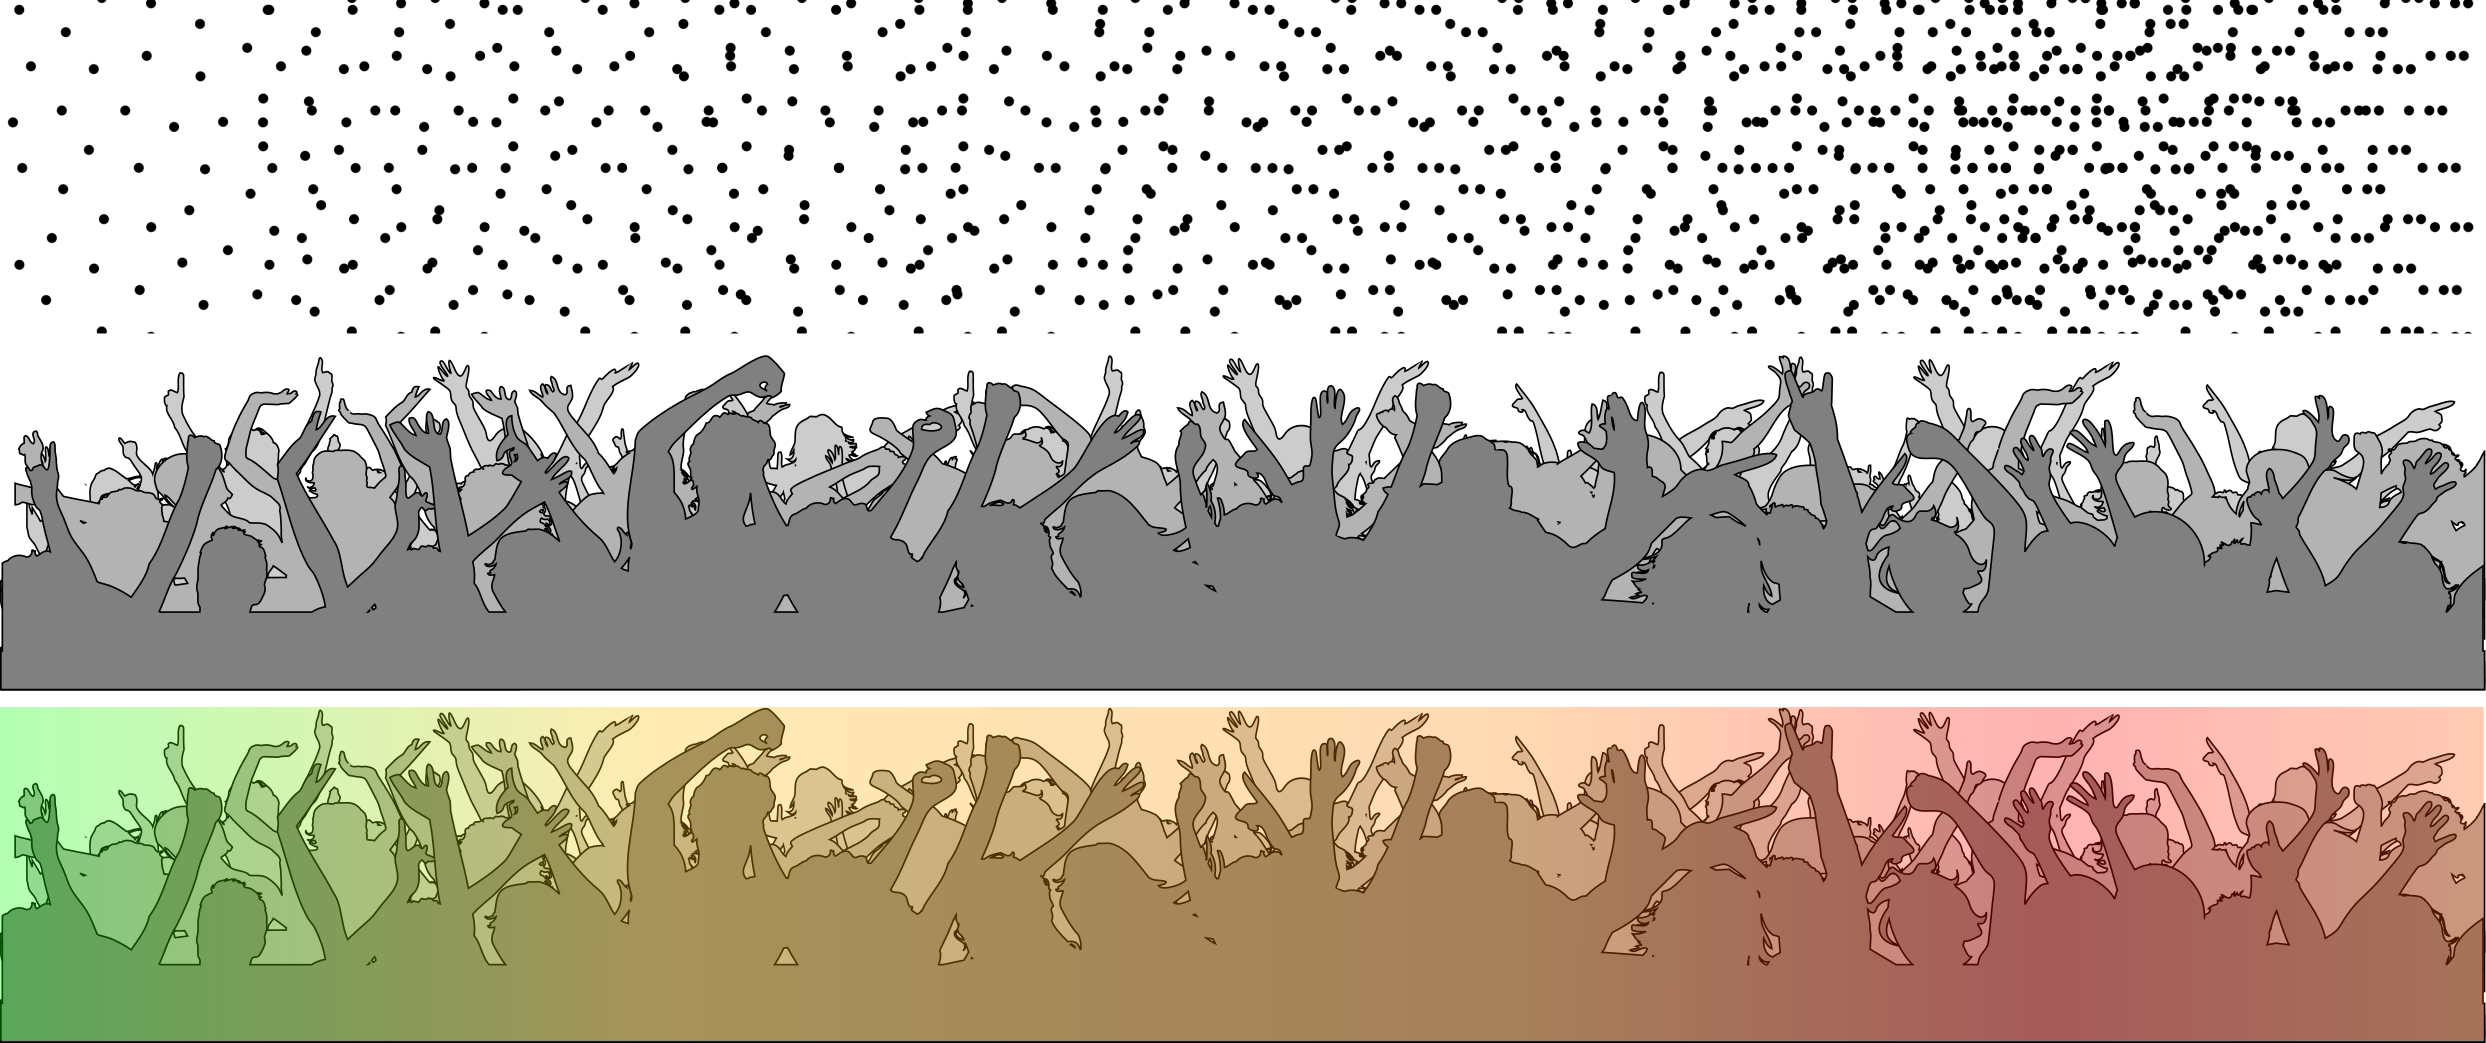
\includegraphics[width=.99\textwidth]{images/crowdar}
  \end{center}
\end{frame}
\begin{frame}{Developer view}
  Crowd detection program development: see the field.
  \begin{center}
    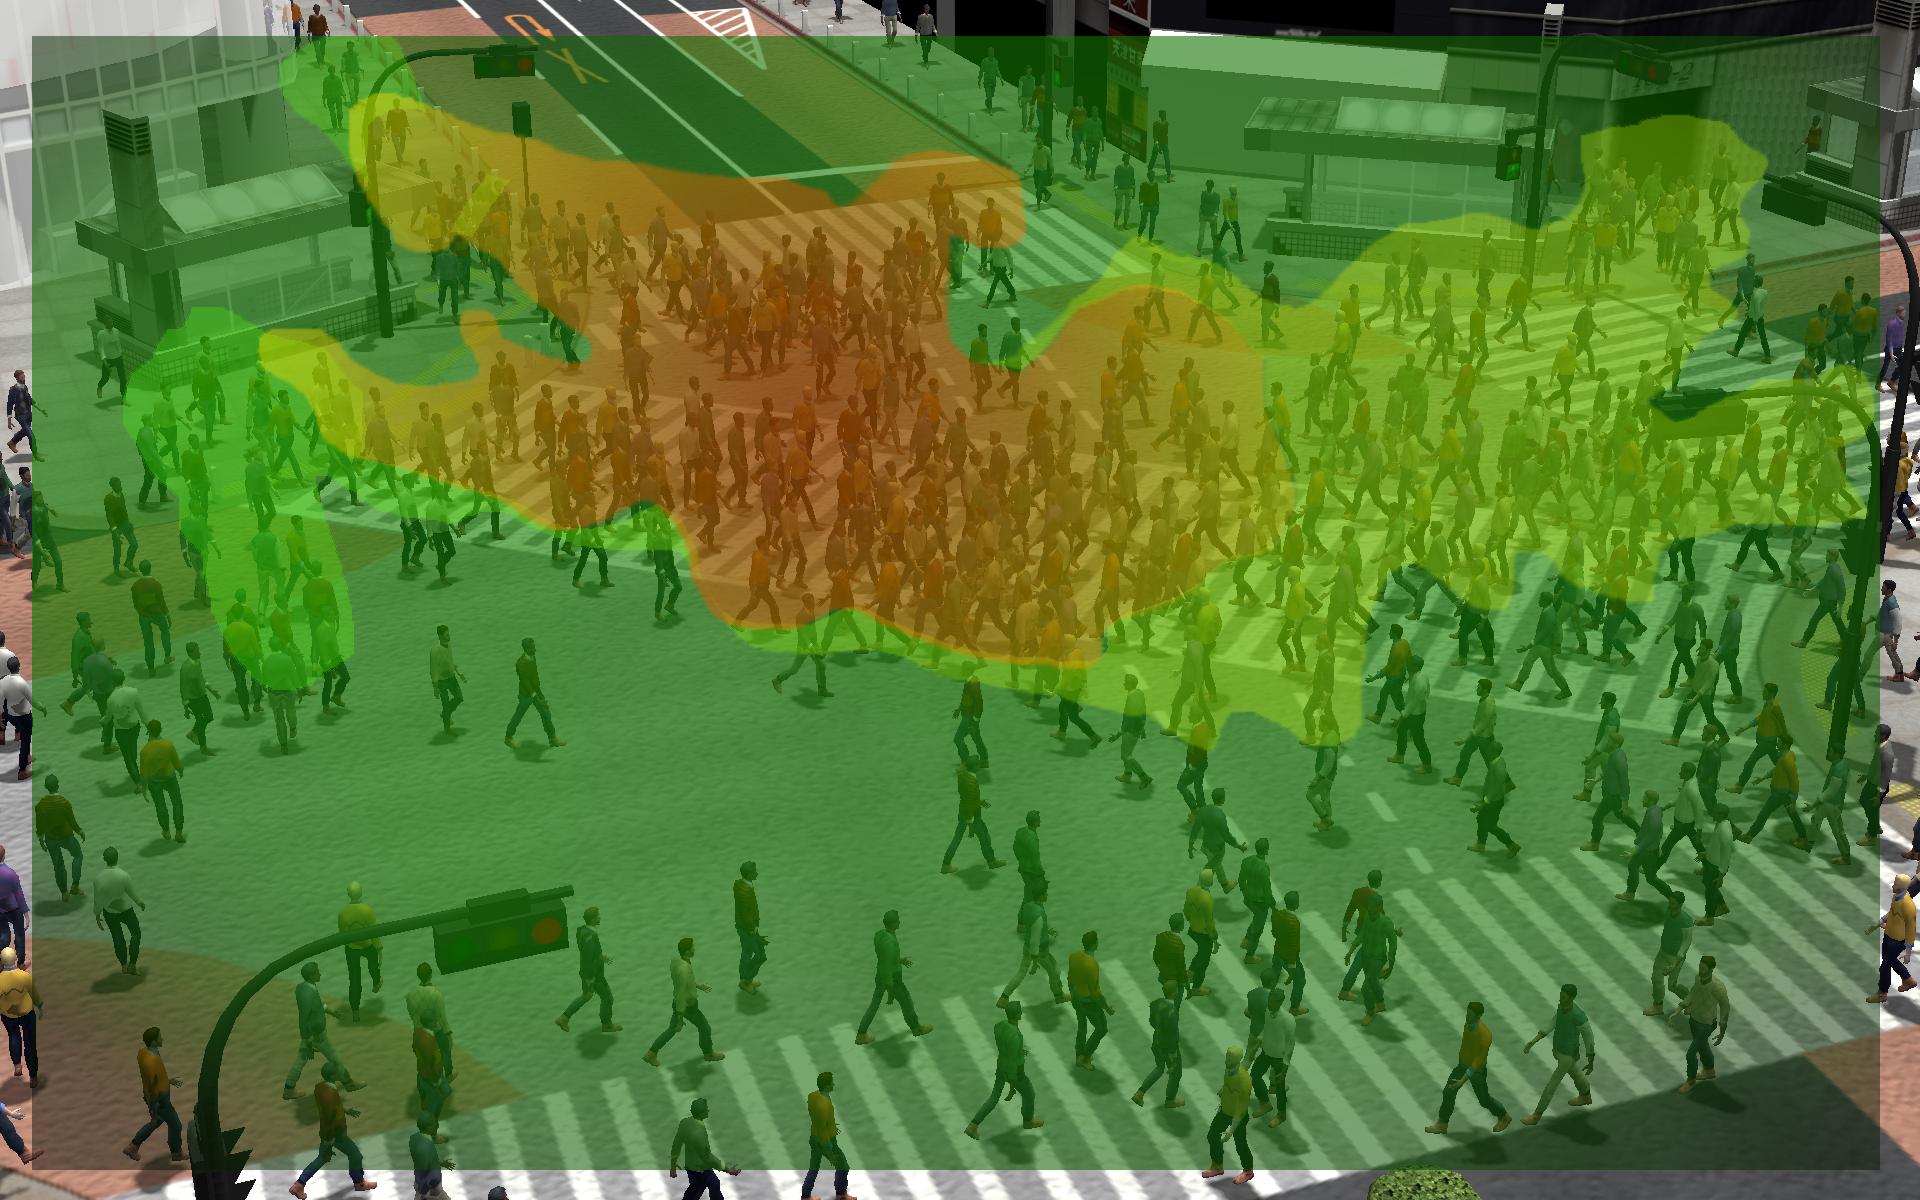
\includegraphics[width=.85\textwidth]{images/crowd01}
  \end{center}
\end{frame}
%-------------------------------------------------------------------------------
\subsection{Augmented reality-based input for CF program}
%-------------------------------------------------------------------------------
\begin{frame}{Weak interaction}
  Provide input to a CF program through AR interaction
  \begin{block} {How}
   \begin{itemize}
    \item Connect the (processed) AR input to the ``sensors'' of a CF program
    \item Requires basically no intervention on the CF program
    \item New information must be added to an existing device participating the aggregate
   \end{itemize}
  \end{block}
  \begin{block} {Why}
   \begin{itemize}
    \item Some system settings could be very naturally set by means of a gesture
   \end{itemize}
  \end{block}
  \begin{block} {Limitations}
   \begin{itemize}
    \item The new information is constrained in a device (a single point in space)
   \end{itemize}
  \end{block}
\end{frame}

\begin{frame}{Strong interaction}
  \begin{center}
    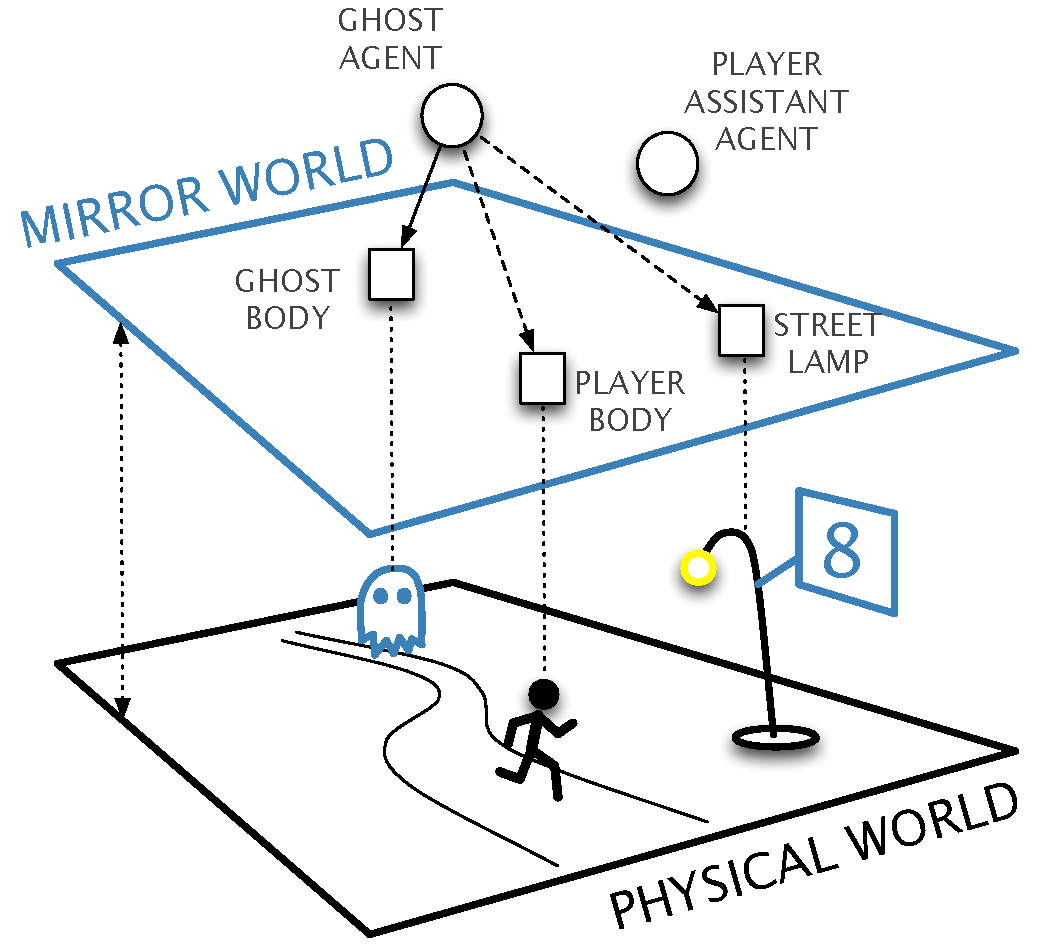
\includegraphics[width=.6\textwidth]{images/game2}
  \end{center}
\end{frame}

\begin{frame}{Strong interaction}
  Inject new information that lives in a ``Mirror World''
  \begin{block} {How}
   \begin{itemize}
    \item Modify the CF program to ``sustain'' the existence of entities in areas where no device is located
    \begin{itemize}
      \item e.g. with a field of mappings between virtual entities and their position
    \end{itemize}
   \end{itemize}
  \end{block}
  \begin{block} {Why}
   \begin{itemize}
    \item Support for highest degree of augmented reality
    \item Mixed real-virtual collective applications
   \end{itemize}
  \end{block}
  \begin{block} {Limitations}
   \begin{itemize}
    \item The program must be conceived with this kind of interaction in mind
    \item Harder to realize
   \end{itemize}
  \end{block}
\end{frame}


%-------------------------------------------------------------------------------
\subsection{Computational fields as enabling technology for AR applications}
%-------------------------------------------------------------------------------
\begin{frame}{A look the other way around}
  We have discussed increasing degrees of interaction between augmented reality and computational fields, up to a ``strong'' interaction, but...
  \begin{block}{}
    ...are computational fields a valid abstraction for creating such programs?
  \end{block}
  \begin{block} {Progression}
   \begin{itemize}
    \item ``Weak'' interaction is almost a free lunch
    \item ``Strong'' interaction seems powerful, but requires CF programs to be designed with AR in mind
    \begin{itemize}
      \item AR is no longer confined to be an I/O component of the system, it impacts the ``business logic'' of the application instead
    \end{itemize}
   \end{itemize}
  \end{block}
\end{frame}

\begin{frame}{Mirror Worlds on Augmented Fields}
  \begin{block}{}
    \begin{itemize}
      \item Basic strategy: 
      \begin{itemize}
        \item Switch from a simple field of mirrored entities to a field of entities with location
        \item Exploit CF programming to keep the entities alive and their status aligned on multiple devices
      \end{itemize}
      \item If entities have their own behavior, mobile code support is required \cite{computationalfields-forte2015}
      \item Reusable building blocks can be exploited in order to devise a ``standard'' solution \cite{IoT2015}
    \end{itemize}
  \end{block}
\end{frame}

%-------------------------------------------------------------------------------
\subsection{Example}
%-------------------------------------------------------------------------------
\begin{frame}{Aggregate triage}
ANGELO
\end{frame}

%===============================================================================
\section{Conclusion}
%===============================================================================
%-------------------------------------------------------------------------------
\subsection{Conclusion and future work}
%-------------------------------------------------------------------------------
\begin{frame}{Conclusion}
  \begin{itemize}
    \item We noted that both computational fields and augmented reality work best in environments densely populated with computational devices
    \item We have explored increasing degrees of integration
    \begin{itemize}
      \item AR as UI $\Rightarrow$ not hard, no change in aggregate programs
      \item Local input from AR devices $\Rightarrow$ still not hard, still no change
      \item Injection of (possibly proactive) augmented entities, $\Rightarrow$ requires CF programs to be properly designed
    \end{itemize}
    \item Modern aggregate programming languages support code mobility and reusability
  \end{itemize}
  \begin{block}{}
    We believe that CF are a promising programming abstraction for supporting AR applications, and languages and technologies are maturing
  \end{block}
  \begin{block}{Future work}
    Build a working demo is the most effective way of experimentally confirm our hypothesis.
  \end{block}
\end{frame}




\section*{\refname}
%===============================================================================
\begin{frame}[allowframebreaks]
%\begin{frame}[t,allowframebreaks]
  \frametitle{\refname}
  \scriptsize
  \bibliographystyle{alpha}
  \bibliography{bibliography}
\end{frame}
\section*{\refname}




\end{document}